\documentclass[titlepage]{article}
\usepackage[utf8]{inputenc}
\usepackage[czech]{babel}
\usepackage{amsmath}
\usepackage{physics}
\usepackage{pdfpages}
\usepackage{graphics}
\usepackage{esint}
\usepackage{graphicx}
\usepackage{auto-pst-pdf} 
\begin{document}
    \begin{titlepage}
        \begin{center}
            \vspace*{1cm}
                
            \Large
            \textbf{LABORATORNÍ CVIČENÍ Z FYZIKY}
                
            \vspace{0.5cm}
            MĚŘENÍ PERMITIVITY DIELEKTRIK
                
            \vspace{1.5cm}
                
            \textbf{Tomáš Kysela}\\
            \textbf{Skupina L1061}
                
            \vfill
                
            \vspace{0.8cm}
            
            
            ČESKÉ VYSOKÉ UČENÍ TECHNICKÉ V PRAZE\\
            FAKULTA ELEKTROTECHNICKÁ\\
            KATEDRA FYZIKY\\
            30. 03. 2021
                
        \end{center}
    \end{titlepage}
    \tableofcontents
    \newpage
    \section{Úvod}
    		Cílem je zjistit permitivitu některých materiálů, konkrétně tedy dielektrik. \newline
    		Dielektrikum (také označován izolant), jež za normálních podmínek proud nevede. Je li ale vložen do elektrického pole (například mezi desky kondenzátoru), permitivita tohoto pole vzroste.
    		
    		\subsection{Gaussova věta}
    			\begin{quote}
    				Tok elektrického pole uzavřenou plochou je v přímém vztahu s náboji uvnitř plochy.
    			\end{quote}
    			Toto lze vyjádřit vzorcem:
    			\begin{equation} 
    				\varoiint_S \vb{E} \cdot d\vb{S} = \frac {Q}{\varepsilon_0}
    			\end{equation}
    			kde E je elektrická intenzita, S gaussovská plocha, Q elektrický náboj a $ \varepsilon_0 $ permitivita vakua.\\
    			Jelikož elektrické pole mezi deskami kondenzátoru se v přítomnosti dielektrika zeslabilo, lze předpokládat že celkový náboj je menší než před vložením. Jelikož ale neklesne na nulu a tudíž je menší než záporný náboj na vodiči. Toto chování lze připodobnit chování vodiče.
    		\subsection{Coulombův zákon}
    			\begin{quote}
    				Mezi dvěma nepohybujícími se náboji působí síla, která je přímo úměrná součinu nábojů a nepřímo úměrná druhé mocnině vzdálenosti mezi nimi. Síla má směr přímky spojující oba náboje.
    			\end{quote}
    			
    			\begin{equation}
    				\vb{F_1} = \frac{1}{4 \pi \varepsilon_0} \frac{q_1 q_2}{r_{12}^2} \vb{e_{12}} = -\vb{F_2}
    			\end{equation}
    			kde $\vb{F_{1,2}}$ jsou síly působící na náboje $q_{1,2}$, $\vb{e_{12}}$ je jednotkový vektor směřující od $q_2$ k $q_1$ a $r_{12}$ je vzdálenost mezi náboji.
    			Zavedeme pojem elektrické pole, které značíme $\vb{E}$ a definujeme jako
    			\begin{equation}
    				\vb{E} = \frac{\vb{F_1}}{q_1}
    			\end{equation}
    			Z rovnic (2) a (3) vyplývá následující rovnice
    			\begin{equation}
    				\vb{E}(1) = \frac{1}{4 \pi \varepsilon_0} \frac{q_2}{r_{12}^2}\vb{e_{12}}
    			\end{equation}
    			
    			Jelikož lze $\vb{e_{12}}$ vyjádřit jako $\frac{r_{12}}{r_{12}}$, lze říci, že pro obecné $\vb{E}(\vb{r})$ platí
    			\begin{equation}
    				\vb{E}(\vb{r}) = \frac{q}{4 \pi \varepsilon_0} \frac{\vb{r}-\vb{r'}}{\abs{\vb{r}-\vb{r'}}^3}
    			\end{equation}
    			kde $\vb{r'}$ je polohový vektor náboje $q$ a $\vb{r}$ polohovým vektorem náboje $q_0$ pro jehož okolí je pole vyšetřováno.
    			
    			Je-li však v okolí náboje $q_0$ dalších nábojů více, je třeba rovnici upravit.
    			\begin{equation}
    				\vb{E}(\vb{r}) = \frac{1}{4 \pi \varepsilon_0} \sum_{i=1}^N \frac{q_i \cdot (\vb{r}-\vb{r_i'})}{\abs{\vb{r}-\vb{r_i'}}^3}
    			\end{equation}
    			Pokud jsou ale okolní náboje příliš hustě namačkané na sebe je třeba využít integrál.
    			\begin{equation}
    				\vb{E}(\vb{r}) = \frac{1}{4 \pi \varepsilon_0} \iint_S \frac{\sigma (\vb{r_i'})  \cdot (\vb{r}-\vb{r_i'})}{\abs{\vb{r}-\vb{r_i'}}^3}\dd{S'}
    			\end{equation}
    			kde S je gaussovská plocha a pro každou její nekonečně malou část platí
    			\begin{equation*}
    				\dd{q} = \sigma \dd{S'} \qq{kde} \sigma = \sigma (\vb{r'}) \qq{je plošná hustota náboje}
    			\end{equation*}
    			
    		\subsection{Kapacita}
    			Nejdříve je třeba zavést pojem elektrické napětí. To definujeme jako práci vykonanou elektrostatickým polem při přemístění jednotkového náboje z  bodu 1 do bodu 2. To lze napsat rovnicí
    			\begin{equation}
    				U = \int^{\vb{r_B}}_{\vb{r_A}}\vb{E}\cdot\dd{\vb{r}}
    			\end{equation}
    			Pro kondenzátor s deskami o velikosti S umístěné ve vzdálenosti d dostaneme
    			\begin{equation}
    				U = \int^d_0\vb{E}\cdot\dd{x} = \int_0^d \frac{\sigma}{\varepsilon_0}\dd{x} = \frac{\sigma d}{\varepsilon_0} = \frac{d}{\varepsilon_0 S}Q
    			\end{equation}
    			
    			Kapacitu následně definujeme jako konstantu úměrnosti a zapisujeme ji vztahem
    			\begin{equation}
    				C = \frac{Q}{U}
    			\end{equation}
    		\subsection{Kondenzátor s dielektrikem}
    			Pokud do kondenzátoru s intenzitou elektrického pole $E_0$ vložíme dielektrikum dostaneme intenzitu elektrické pole $E = E_0-E'$. Následně zavádíme relativní permitivitu $\varepsilon_r$ definované jako
    			\begin{equation}
    				\varepsilon_r = \frac{E_0}{E} = \frac{E_0}{E_0 - E'}
    			\end{equation}
    			a následně
    			\begin{equation}
    				U = \frac{d}{\varepsilon_0 \varepsilon_r S}Q
    			\end{equation}
    			\begin{equation}
    				C = \frac{\varepsilon_0 \varepsilon_r S}{d}
    			\end{equation}
    	\section{Úkoly}
    		Je třeba naměřit následující hodnoty:
    		\begin{itemize}
    		\item $U$ Napětí na kondenzátoru s vloženým dielektrikem
    		\item $U_0$ Referenční napětí na kondenzátoru
    		\end{itemize}
    	\section{Popis experimentu}
    		\subsection{Použité přístroje}
    		\begin{tabular}{| c | c | c |}
    			\hline
    			\textbf{Přístroj} & \textbf{Výrobce} & \textbf{Rozlišení / TP / Hodnota}\\
			\hline
			\hline
			Voltmetr & PHYWE & TP 2.5\\
			\hline
			Referenční kondenzátor & & 216 nF\\
			\hline
			Deskový kondenzátor pro měření materiálu & & \\
			\hline
			Nonius k kondenzátoru & PHYWE & 0.1mm\\
			\hline
			Měřící zesilovač & PHYWE & \\
			\hline
			HV zdroj napětí & PHYWE & 0 - 10 kV\\
			\hline
    		\end{tabular}
    	\section{Výsledky}
    		\subsection{Naměřené hodnoty a výpočet Cx}
    			\begin{align*}
    				u(U_{xi}) &= \frac{rozsah \cdot \frac{2.5}{100}}{\sqrt{3}} = rozsah \cdot 0.0144338\\
    				Q_i &= C_0 \cdot U_{xi}\\
    				u(Q_i) &= \sqrt{(\frac{\dd{Q}}{\dd{U_{xi}}})^2u^2(U_{xi})} = C_0 \cdot u(U_{xi})\\
    				C_{xi} &= \frac{Q_i}{U}
    			\end{align*}
\begin{tabular}{|c|c|c|c|c|c|c|} 
\hline
\textbf{Nastaveno} & \textbf{Měřeno} & \textbf{Rozsah} &            &             &               &              \\ 
\hline
\textbf{ U }       & $U_x$           & $U_x$           & $u(U_x)$   & \textbf{Q}  & \textbf{u(Q)} & $C_x$        \\ 
\hline
\textbf{ kV }      & \textbf{V }     & \textbf{V }     & \textbf{V} & \textbf{nC} & \textbf{nC}   & \textbf{pF}  \\ 
\hline\hline
\multicolumn{7}{|c|}{\textbf{PVC}}                                                                               \\ 
\hline\hline
0.5                & 0.51            & 1               & 0.0144338  & 110.16      & 3.1177008     & 220.32       \\ 
\hline
1.0                & 0.98            & 1               & 0.0144338  & 211.68      & 3.1177008     & 211.68       \\ 
\hline
1.5                & 1.45            & 3               & 0.0433014  & 313.20      & 9.3531024     & 208.80       \\ 
\hline
2.0                & 1.90            & 3               & 0.0433014  & 410.40      & 9.3531024     & 205.20       \\ 
\hline
2.5                & 2.30            & 3               & 0.0433014  & 496.80      & 9.3531024     & 198.72       \\ 
\hline
3.0                & 2.75            & 3               & 0.0433014  & 594.00      & 31.177008~    & 198.00       \\ 
\hline
3.5                & 3.30            & 10              & 0.1443380  & 712.80      & 31.177008~    & 203.66       \\ 
\hline
4.0                & 3.80            & 10              & 0.1443380  & 820.80      & 31.177008~    & 205.20       \\ 
\hline
4.5                & 4.30            & 10              & 0.1443380  & 928.80      & 31.177008     & 206.40       \\ 
\hline
5.0                & 4.70            & 10              & 0.1443380  & 1015.20     & 31.177008     & 203.04       \\ 
\hline\hline
\multicolumn{7}{|c|}{\textbf{Vzduch}}                                                                            \\ 
\hline\hline
0.5                & 0.19            & 0.3             & 0.0043301  & 41.04       & 0.93531024    & 82.08        \\ 
\hline
1.0                & 0.36            & 1               & 0.0144338  & 77.76       & 3.1177008     & 77.76        \\ 
\hline
1.5                & 0.52            & 1               & 0.0144338  & 112.32      & 3.1177008     & 74.88        \\ 
\hline
2.0                & 0.67            & 1               & 0.0144338  & 144.72      & 3.1177008     & 72.36        \\ 
\hline
2.5                & 0.84            & 1               & 0.0144338  & 181.44      & 3.1177008     & 72.58        \\ 
\hline
3.0                & 1.00            & 3               & 0.0433014  & 216.00      & 9.3531024     & 72.00        \\ 
\hline
3.5                & 1.15            & 3               & 0.0433014  & 248.40      & 9.3531024     & 70.97        \\ 
\hline
4.0                & 1.35            & 3               & 0.0433014  & 291.60      & 9.3531024     & 72.90        \\ 
\hline
4.5                & 1.50            & 3               & 0.0433014  & 324.00      & 9.3531024     & 72.00        \\ 
\hline
5.0                & 1.60            & 3               & 0.0433014  & 345.60      & 9.3531024     & 69.12        \\
\hline
\end{tabular}
    				
    			\includegraphics[width=3in, angle=-90, origin=c]{gr-graf-1620764421-color.ps}
    			\begin{align*}
    				C_{PVC} &= 206.10 pF\\
    				u(C_{PVC}) &=  5.43818pF\\
    				C_{vzduch} &= 73.66pF\\
    				u(C_{vzduch}) &= 2.14316pF
    			\end{align*}
    		\subsection{Výpočet relativní permitivity}
    			\begin{align*}
    				\varepsilon_r &= \frac{C_{PVC}}{C_{vzduch}}\\
    				\varepsilon_r &= \frac{206.10 pF}{73.66pF} = 2.798\\
    				u(\varepsilon_r) &= \sqrt{(\frac{\dd{\varepsilon_r}}{\dd{C_{PVC}}})^2u^2(C_{PVC}) + (\frac{\dd{\varepsilon_r}}{\dd{C_{vzduch}}})^2u^2(C_{vzduch})}\\
    				u(\varepsilon_r) &= \sqrt{(\frac{u(C_{PVC})}{C_{vzduch}})^2 + (\frac{C_{PVC} \cdot u(C_{vzduch})}{C_{vzduch}^2})^2}\\
    				u(\varepsilon_r) &= \sqrt{(\frac{5.43818pF}{73.66pF})^2 + (\frac{206.10 pF \cdot 2.14316pF}{73.66^2pF})^2} = 0.1099\\
    			\end{align*}
    			Výsledek:
    				$$ \varepsilon_r = 2.80 \pm 0.11 $$
  	\section{Diskuze}
  		Výsledek je uvěřitelný, nikoli však přesný. Očekávaný výsledek byl v rozmezí 3.6-4. Této odchylky jsem se nejspíše dopustil nepřesnostmi v počítání a zaokrouhlením desetinných míst.
  	\section{Závěry}
  		Zvolený postup měření byl správný. Nepřesností v následném výpočtu se ale výsledek $$ \varepsilon_r = 2.80 \pm 0.11 $$ liší o zhruba 1 od výsledku očekávaného.
  	\section{Seznam literatury}
  		[1] ŠANDEROVÁ, Věra a Zdeněk KYNCL. Fyzika I. 3. Praha: Ediční středisko ČVUT, 1987.\newline
		[2] FEYNMAN, Richard Phillips, Robert B. LEIGHTON a Matthew SANDS. Feynmanovy přednášky z fyziky s řešenými příklady. Havlíčkův Brod: Fragment, 2000. ISBN 80-7200-405-0.\newline
		[3] Červenka: Zpracování fyzikálních měření,\newline https://planck.fel.cvut.cz/praktikum/downloads/navody/zpracdat.pdf\newline
		[4] Červenka: Laboratorní úloha: Měření permitivity dielektrik,\newline https://planck.fel.cvut.cz/praktikum/downloads/navody/permitivita.pdf
\end{document}